\section{Section 4}

Figure 5 shows that the percentage of services having standards are
increasing over the past few year. For example, among the 1637 services 
available for 2022 to 2023, there were 928 of them having standards, 
which is 56.7\% for a total of 2,280 service standards. Meanwhile, more
than 50\% of the service standard targets were met after 2020. One can
see an improvment on the performance of the government in terms of meeting
the service standard target. In particular, 1348 out of 2280 standard 
targets were met during 2022 to 2023, counting for 59.1\% which is the 
highest over the past few years.

\begin{figure}
    \centering
    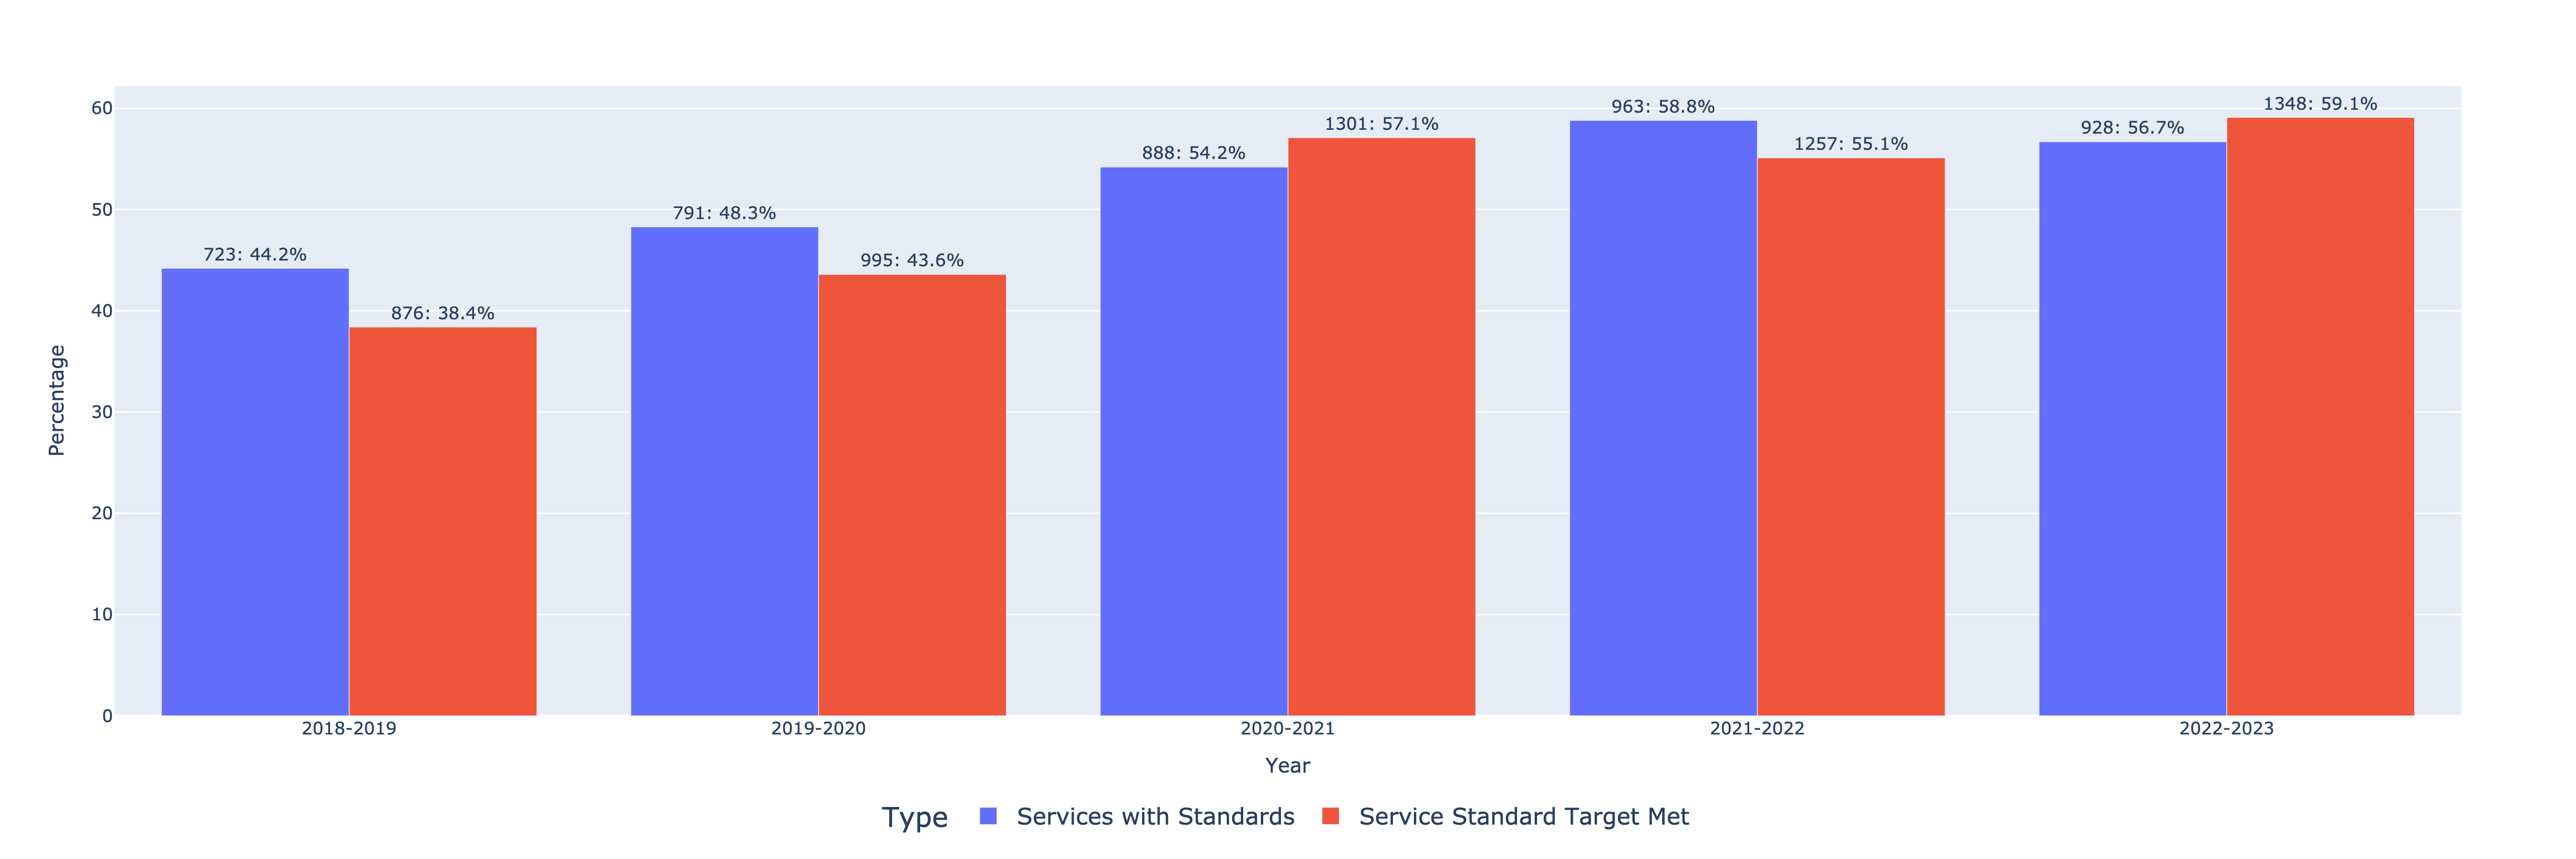
\includegraphics[width=1\linewidth]{StdWithTarget.png}
    \caption{\label{fig:Std}Percentage of Services with Standards and Standards with Target Met}
\end{figure}
